\chapter{Design and Implementation}
\label{chap:design-and-implementation}
\vspace{-0.75cm}
\centerline{\rule{149mm}{.02in}}
\vspace{0.75cm}

This section describes how each structure was implemented and documents the low-level optimisation efforts that went into accelerating the structures.

TODO: add mention of how times are retrieved (more detail in detail...)

\section{Evaluation Framework}

Evaluation forms a major part of this project. It was decided a framework should be used to streamline this process and reduce the time it takes to generate the measurements required for evaluation.  The framework was created because performance analysis would be done very frequently, multiple times per iteration. Manually timing and profiling the code each time is time-consuming and error-prone. Putting more effort initially into creating a system that allows large sets of operations and index structures to be tested at once can save a significant amount of time later on. No tool for this task existed, so it was created for this project.

The evaluation framework takes a specification containing all the datasets and index structures to test, and executes the Insert-Query-Delete operation list for the given datasets on all specified structures. The output is a set of text files containing the performance measures described in Section \ref{sec:performance-measures}. The text files the executable produces are fed into Python scripts to automatically generate tables and plots.

There are three core modules of the framework, which are shown in Figure \ref{fig:evaluation-framework} and listed below:
\begin{itemize}
	\item \texttt{data} -- library that contains standard data types used throughout framework and index structures, as well as dataset generators/loaders
	\item \texttt{index\_structure} -- library that contains every index structure implemented in the project
	\item \texttt{evaluator} -- executable program that takes specification file and runs a set of automated performance tests to produce text files containing evaluation measures
\end{itemize}

\begin{figure}
	\centering
	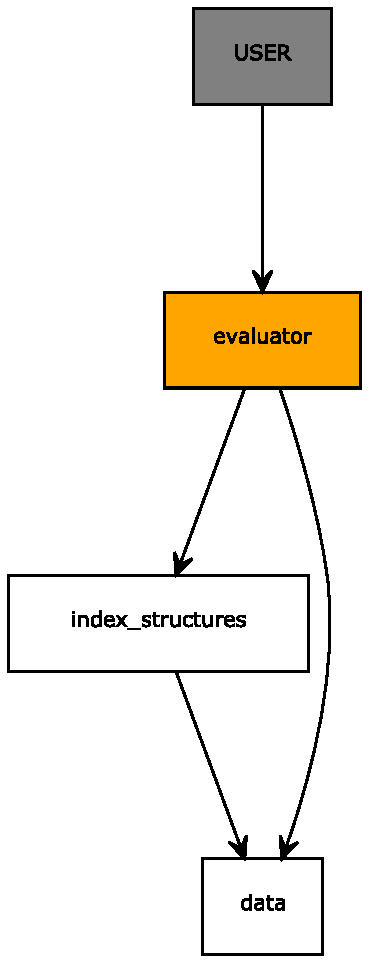
\includegraphics[scale=0.6]{figures/evaluation_framework.pdf}
	\caption{Modules of Evaluation Framework}
	\label{fig:evaluation-framework}
\end{figure}

\section{Baseline Implementations}

Sequential scan was implemented using the C++ container \texttt{std::vector}, a dynamically resizeable array.  Point queries are performed in $O(n)$ time, as the query iterates through the array sequentially until the given point is found or the end of the array is reached. The structure must check if a point exists in the structure before inserting it, making \texttt{insert} take $O(n)$. \texttt{delete} is a standard array deletion, making it an $O(n)$ operation.

The octree variant implemented is a bucket PR octree. The structure partitions the underlying data space into uniformly sized boxes, without using the points as pivots (unlike point quadtrees). It is a bucket octree because \textit{multiple} points can be stored in a single leaf node. The octree dynamically decomposes spatial regions based on its current contents. When the number of points in a leaf node exceeds a certain number, say $M$, then the region represented by the leaf is sub-divided, creating $2^d$ children. The $M + 1$ points are then scattered across the children. Therefore, dense regions of space have a finer decomposition than sparse regions.

When a point is deleted from a leaf, the leaf's contents and its siblings are checked. If all of these nodes are empty, they are removed and the sub-regions are collapsed into a single node representing the whole region. If the collapsed node and its siblings are empty, then they are collapsed into their parent. This is repeated until there is a parent whose children contain at least one point.

\section{Compiler Optimisation}

GCC\footnote{GCC, the GNU Compiler Collection -- \url{http://gcc.gnu.org/}} was the C++ compiler used in this project. GCC can automatically modify the compiled program to make it more efficient on the target platform. There are multiple optimisation levels, going from 0 (no optimisation) to 3 (maximum optimisation).

Table \ref{tab:compiler-optimisation} shows the execution times of the two baselines on 10,000 random 10D points, when level 0 and level 3 optimisation is used. Level 3 optimisation consistently increased the structures, showing that the potential speed gains are huge. For example, the octree's point queries are approximately $6.5$ times faster, just by enabling level 3 optimisation.  In order to make the structures as fast as possible, level 3 optimisation will be used when compiling all index structures in the project.

\begin{table}
	\centering
	\begin{tabular}{|l|l|l|l|}
		\hline
		\textbf{Structure} & \textbf{Operation} & \textbf{Level 0} & \textbf{Level 3} \\
		\hline
		\multirow{ 4}{*}{Sequential Scan} & Insert & 1.33509 & 0.111372 \\
		 & Delete & 5.29548 & 0.623759 \\
		 & Point Query & 1.33468 & 0.111909 \\
		\hline
		\multirow{ 4}{*}{Octree} & Insert & 1.23108 & 0.243256 \\
		 & Delete & 0.73156 & 0.13589 \\
		 & Point Query & 0.559736 & 0.0860926 \\
		 \hline
	\end{tabular}
	\caption{Total Execution Time (in Seconds) of Structure Operations With Different Levels of Compiler Optimisation (10,000 10D Random Points)}
	\label{tab:compiler-optimisation}
\end{table}

\section{Hash-Based Structures}
\label{sec:iteration1}

This section discusses the low-level implementation details of the hash-based structures developed in this project. Multiple implementations of are developed and analysed to determine which is the fastest.

\subsection{Initial Hash Structure Implementation}

The Pyramid Tree, Pseudo-Pyramid Tree and Bit Hash are essentially hashing functions, where the one-dimensional value acts as the hash to use when searching a hash table.
An implementation of a generic hash structure, where the hashing function can be varied, will be created for these hash-based structures to use. The structure stores all the points in a single array, which hashes each point to an integer representation that acts as the key to a bucket stored in a hash map (specifically \texttt{boost::unordered\_map}, part of the Boost\footnote{\url{http://www.boost.org/}} library). A bucket is an array that contains indices to points in the large array.

To determine if a point $p$ is stored in the structure, $p$ is first hashed into its one-dimensional representation. The corresponding bucket is then sequentially scanned until the point is found or the end of the bucket is reached. To reduce the number of floating point comparisons, especially for large $d$, the \textit{sums} of each point are stored when they are inserted. This way, a $O(d)$ point comparison only needs to be performed if the $O(1)$ point sum comparison passes.

To delete a point $p$, the point is first hashed and the bucket containing the point is found. The index in the bucket pointing to $p$ is removed, but the actual point itself is not removed from the point array. This will not release memory now unused by the deleted point. This is not suitable if the structure is used as part of a long-running process because there is the potential to run out of memory. One of the core assumptions of this project is that data may be dynamic, meaning points may be inserted and deleted frequently. For this reason, memory must be released when deleting points.

The \textbf{Rebuild Hash Structure} releases memory when $R$ points have been removed, where $R$ is a configurable parameter. When a point is removed, the index of the element storing the point is marked. Once $R$ elements are marked, a rebuild procedure is performed. The entire hash structure is rebuilt by first clearing the structure and then inserting all the points \textit{not} marked for deletion. $n - R + 1$ points will be re-inserted and insertion in the worst case is $O(n)$, meaning the worst case complexity of \texttt{delete} is $O((n - R)n)$. The larger $R$ is, the less often the rebuild procedure executes, but a larger amount of allocated memory goes unused at a time.

\subsection{Bucket Implementation}
\label{sec:bucket-hash-structure}

The rebuild implementation stores indices in buckets, meaning that points in the same bucket may not be stored contiguously in memory. Searching a bucket in the rebuild implementation is likely to incur a lot of cache misses, because accessing a point will incur random access into the single point array. Reading a point in a bucket also requires the CPU to fetch two elements from main memory -- the index of the point and the point itself. Furthermore, having a large point array makes \texttt{delete} operations more complicated because the indices stored in buckets must be maintained.

\textbf{Bucket Hash Structure} is another implementation that was created which does not use a single array to store the points. Buckets contain actual points instead of indices to them. This should reduce cache misses since point array is searched sequentially. No rebuild procedure is necessary because the memory for a point is released immediately after it is removed, by simply erasing it from the corresponding bucket's array (which is much smaller than an array containing \textit{all} the points). The order the points are stored in a bucket do not matter, so the \textit{erase-remove} idiom\footnote{\url{http://en.cppreference.com/w/cpp/algorithm/remove}} has been used to delete elements from the bucket arrays.

\subsection{Splay Tree Variant}

The \textbf{Splay Hash Structure} uses a splay tree as the underlying one-dimensional index structure, instead of a hash map. The splay tree is a self-adjusting binary search tree that uses a a heuristic to allow faster access to recently accessed elements. \cite{splay-tree}. Through amortised analysis and empirical experiments, it has been shown splay trees can be more efficient than standard binary trees for a series of non-random operations \cite{splay-tree}, despite the worst case bound being worse than binary search trees.

Nodes in the Splay Pseudo-Pyramid Tree correspond to individual buckets in the Bucket Hash Structure. Since the splay tree is implemented as a collection of heap-allocated nodes, deletions are cheap as a low amount of memory needs to be de-allocated per \texttt{delete} operation. This, combined with the self-adjusting nature of the splay tree, could produce an more efficient  implementation for non-random operations used in real applications.

\subsection{Cache Misses}

Table \ref{tab:perf1-cache-hit-rate} displays the cache miss rate when inserting 10,000 10D random points into each implementation, using the Pseudo-Pyramid Tree hashing function. Notice how the Rebuild Hash Structure, which stores indices in each bucket, has the highest cache miss rate. The Bucket Hash Structure incurs the least amount of cache misses, showing how contiguous memory storage can have a significant impact on cache misses.

\begin{table}
	\centering
	\begin{tabular}{|r|l|}
		\hline
		\textbf{Structure} & \textbf{Cache Miss Rate (\%) (2 dp)} \\
		\hline
		Rebuild Hash & 4.62 \\
		Bucket Hash & 0.28 \\
		Splay Hash & 0.59 \\
		\hline
	\end{tabular}
	\caption{Cache Hit Rate for \texttt{insert} Operations with Hash Structure Implementation Using Pseudo-Pyramid Tree Hashing Function (10,000 10D Random Points)}
	\label{tab:perf1-cache-hit-rate}
\end{table}

\subsection{Fastest Implementation}

Table \ref{tab:hash-implementation-speeds} shows the execution times of each operation on each of the structures, for 10,000 random 10D points. The Splay Hash Structure is the slowest for insertions and queries. Rebuild Hash Structure has the deletions (due to the rebuild procedure), but its insertion and query performance almost matches the Bucket Hash Structure. The Bucket Hash Structure outperforms the other implementations, coinciding with their cache miss rates. All hash-based structures will the Bucket Hash Structure implementation, with the hash function varying.

\begin{table}
	\centering
	\begin{tabular}{|r|l|l|l|}
	\hline
	\textbf{Structure} & \textbf{Insert} & \textbf{Delete} & \textbf{Point Query}  \\
	\hline
	Rebuild Hash & 0.002467 & 0.019018 & 0.000977 \\
	Bucket Hash & 0.003546 & 0.001448 & 0.000958 \\
	Splay Hash &  0.005368 & 0.002074 &  0.001542 \\
	\hline
	\end{tabular}
	\caption{Execution Time (in seconds) of Hash Structure Implementations Using Pseudo-Pyramid Tree Hashing Function (10,000 10D Random Points)}
	\label{tab:hash-implementation-speeds}
\end{table}

\subsection{B${}^+$-Tree for Underlying Structure of Pyramid Tree}

Berchtold et al. originally used a B${}^{+}$-tree when developing the Pyramid Tree \cite{pyramid-tree}. Using the same underlying search structure allows a more fair comparison of the Pyramid Tree's performance to the literature to be made. Two B${}^{+}$-tree implementations, bpt\cite{bpt} and cpp-btree\cite{cpp-btree}, were tested.

Table \ref{tab:hashtable-bplus-time-comparison} provides total execution times of each operation using \texttt{boost::unordered\_map} and the two B${}^{+}$-tree implementations, measured using 10,000 10D random points. There is a noticeable difference between the speed of the hash table and B${}^{+}$-tree implementations. This matches the theoretical performance analyses of the two structures, where it is shown that hash tables and B${}^{+}$-trees have amortised $O(1)$ and $O(\log n)$ operations respectively. After profiling, it was discovered the main cause of the decrease in speed was the additional overhead incurred by splitting and merging nodes in the B${}^{+}$-tree. Based on these results, it has been decided to continue using the hash table as the underlying search structure for the Pyramid Tree.

\begin{table}
	\centering
	\begin{tabular}{|r|r|l|l|}
		\hline
		\textbf{Operation} & \texttt{boost::unordered\_map} & bpt & cpp-btree  \\
		\hline
		Delete & 0.002206 & 0.004544 & 0.003617 \\
		Insert & 0.005275 & 0.010445 & 0.012766 \\
		Point Query & 0.001534 & 0.002501 & 0.002808 \\
		\hline
	\end{tabular}
	\caption{Total Execution Time (in Seconds) of Pyramid Tree With Different Underlying 1D Index Structures (10,000 10D Random Points)}
	\label{tab:hashtable-bplus-time-comparison}
\end{table}

\section{SSE Optimisation}

Point equality tests have been accelerated using SSE. Considering point equality is used throughout all the index structures, there should be some noticeable speed gains in the structures themselves. It is also possible to parallelise the hashing functions used in this project. For this report, the Pyramid tree hashing function is considered. Both this hashing function and point equality are executed in $O(d)$ time. In both operations there is loop which iterates once for each dimension, where each iteration is independent of the others. If 32-bit floating point numbers are used, then four dimensions can be processed at once using 128 bit SSE registers. If the number of dimensions is less than four, there is little benefit using SSE. When $d<4$, the structures use the sequential version of the code instead.

Table \ref{tab:pyramid-sse} shows the execution times of the Pyramid Tree with and without SSE optimisation for its hash function and point equality. Across all three operations, the average speedup is approximately $1.37$ when there are 10 dimensions. Considering the ideal speedup is 4, it was expected the speed up would be higher. Nevertheless, parallelising point equality consistently achieves speed up for all structures. Other parts of the implementations have been accelerated using SSE, but for brevity have not been included in this report.

\begin{table}
	\centering
	\begin{tabular}{|r|l|l|}
		\hline
		\textbf{Operation} & \textbf{Without SSE} & \textbf{With SSE} \\
		\hline
		Delete & 0.002194 & 0.001613 \\
		Insert & 0.005188 & 0.003856 \\
		Point Query & 0.001577 & 0.001122 \\
		\hline
	\end{tabular}
	\caption{Total Execution Time (in seconds) of Bucket Hash Structure Using Pyramid Tree Hashing Function, With and Without SSE Optimisation (10,000 10D Random Points)}
	\label{tab:pyramid-sse}
\end{table}

\section{$kd$-tree Implementation}

The point $kd$-tree variant described in Section \ref{sec:kd-tree-detail} was implemented. Each node is represented as a C-struct which stores a single point as well as pointers to its children. Every node is allocated using a call to \texttt{malloc()}, which allocates enough memory on the heap to store the node. This means each node may reside in different areas of the heap, resulting in fragmented memory. Array-based implementations that store $kd$-tree contiguously in memory exist, but this project will not explore these due to time constraints.

\section{Conclusion}

TODO